%%%%%%%%%%%%%%%%%%%%%%%%%%%%%%%%%%%%%%%%%
% Beamer Presentation
% LaTeX Template
% Version 1.0 (10/11/12)
%
% This template has been downloaded from:
% http://www.LaTeXTemplates.com
%
% License:
% CC BY-NC-SA 3.0 (http://creativecommons.org/licenses/by-nc-sa/3.0/)
%
%%%%%%%%%%%%%%%%%%%%%%%%%%%%%%%%%%%%%%%%%

%----------------------------------------------------------------------------------------
%	PACKAGES AND THEMES
%----------------------------------------------------------------------------------------

\documentclass[handout]{beamer}

\mode<presentation> {

% The Beamer class comes with a number of default slide themes
% which change the colors and layouts of slides. Below this is a list
% of all the themes, uncomment each in turn to see what they look like.

%\usetheme{default}
%\usetheme{AnnArbor}
%\usetheme{Antibes}
%\usetheme{Bergen}
%\usetheme{Berkeley}
%\usetheme{Berlin}
%\usetheme{Boadilla}
%\usetheme{CambridgeUS}
%\usetheme{Copenhagen}
%\usetheme{Darmstadt}
%\usetheme{Dresden}
%\usetheme{Frankfurt}
%\usetheme{Goettingen}
%\usetheme{Hannover}
%\usetheme{Ilmenau}
%\usetheme{JuanLesPins}
%\usetheme{Luebeck}
\usetheme{Madrid}
%\usetheme{Malmoe}
%\usetheme{Marburg}
%\usetheme{Montpellier}
%\usetheme{PaloAlto}
%\usetheme{Pittsburgh}
%\usetheme{Rochester}
%\usetheme{Singapore}
%\usetheme{Szeged}
%\usetheme{Warsaw}

% As well as themes, the Beamer class has a number of color themes
% for any slide theme. Uncomment each of these in turn to see how it
% changes the colors of your current slide theme.

%\usecolortheme{albatross}
%\usecolortheme{beaver}
%\usecolortheme{beetle}
%\usecolortheme{crane}
%\usecolortheme{dolphin}
%\usecolortheme{dove}
%\usecolortheme{fly}
%\usecolortheme{lily}
%\usecolortheme{orchid}
%\usecolortheme{rose}
%\usecolortheme{seagull}
%\usecolortheme{seahorse}
%\usecolortheme{whale}
%\usecolortheme{wolverine}

%\setbeamertemplate{footline} % To remove the footer line in all slides uncomment this line
%\setbeamertemplate{footline}[page number] % To replace the footer line in all slides with a simple slide count uncomment this line

%\setbeamertemplate{navigation symbols}{} % To remove the navigation symbols from the bottom of all slides uncomment this line
}

\usepackage{graphicx} % Allows including images
\usepackage{booktabs} % Allows the use of \toprule, \midrule and \bottomrule in tables
\usepackage{cool}
\usepackage{amsmath}
\usepackage{amssymb}
\usepackage{bm}
\usepackage{physics}
\usepackage{hyperref}
\usepackage{listings}
\usepackage{enumerate}

\newcommand{\prob}{\mathcal{P}}
\newcommand{\rew}{\mathcal{R}}
\newcommand{\states}{\mathcal{S}}
\newcommand{\actions}{\mathcal{S}}

\DeclareMathOperator*{\argmin}{arg\,min}
\DeclareMathOperator*{\argmax}{arg\,max}

\newcommand{\bvpi}{\bm{V}^{\pi}}
\newcommand{\bvs}{\bm{V}^*}
\newcommand{\bbpi}{\bm{B}^{\pi}}
\newcommand{\bbs}{\bm{B}^*}
\newcommand{\bv}{\bm{V}}

%----------------------------------------------------------------------------------------
%	TITLE PAGE
%----------------------------------------------------------------------------------------

\title[RL Prediction Chapter]{A Guided Tour of \href{http://stanford.edu/~ashlearn/RLForFinanceBook/book.pdf}{\underline{\textcolor{yellow}{Chapter 9}}}: \\ Reinforcement Learning for Prediction} % The short title appears at the bottom of every slide, the full title is only on the title page

\author{Ashwin Rao} % Your name
\institute[Stanford] % Your institution as it will appear on the bottom of every slide, may be shorthand to save space
{ICME, Stanford University
 % Your institution for the title page
}

\date % Date, can be changed to a custom date

\begin{document}
\lstset{language=Python}  
\begin{frame}
\titlepage % Print the title page as the first slide
\end{frame}

% \begin{frame}
% \frametitle{Overview} % Table of contents slide, comment this block out to remove it
% \tableofcontents % Throughout your presentation, if you choose to use \section{} and \subsection{} commands, these will automatically be printed on this slide as an overview of your presentation
% \end{frame}

\begin{frame}
\frametitle{RL does not have access to a probability model}
\begin{itemize}[<+->]
\item DP/ADP assume access to probability model (knowledge of $\mathcal{P}_R$)
\item Often in real-world, we do not have access to these probabilities
\item Which means we'd need to {\em interact} with the {\em actual environment}
\item {Actual Environment} serves up individual experiences, not probabilities
\item Even if MDP model is available, model updates can be challenging
\item Often real-world models end up being too large or too complex
\item Sometimes estimating a {\em sampling model} is much more feasible
\item So RL interacts with either {\em actual} or {\em simulated} environment
\item Either way, we receive {\em individual experiences} of next state and reward
\item RL learns Value Functions from a stream of individual experiences
\item How does RL solve Prediction and Control with such limited access?
 \end{itemize}
\end{frame}

\begin{frame}
\frametitle{The RL Approach}
\begin{itemize}[<+->]
\item Like humans/animals, RL doesn't aim to estimate probability model
\item Rather, RL is a ``trial-and-error'' approach to linking actions to returns
\item This is hard because actions have overlapping reward sequences
\item Also, sometimes actions result in {\em delayed rewards}
\item The key is incrementally updating $Q$-Value Function from experiences
\item Appropriate Approximation of $Q$-Value Function is also key to success
\item RL algorithms are founded on the {\em Bellman Equations}
\item Moreover, RL Control is based on {\em Generalized Policy Iteration}
\item This lecture/chapter focuses on RL for Prediction
\end{itemize}
\end{frame}


\begin{frame}
\frametitle{RL for Prediction}
\pause
\begin{itemize}[<+->]
\item Prediction: Problem of estimating MDP Value Function for a policy $\pi$
\item Equivalently, problem of estimating $\pi$-implied MRP's Value Function
\item Assume interface serves an {\em atomic experience} of (next state, reward)
\item Interacting with this interface repeatedly provides a {\em trace experience}
$$S_0, R_1, S_1, R_2, S_2, \ldots$$
\item {\em Value Function} $V: \mathcal{N} \rightarrow \mathbb{R}$ of an MRP is defined as:
$$V(s) = \mathbb{E}[G_t|S_t = s] \text{ for all } s \in \mathcal{N}, \text{ for all } t = 0, 1, 2, \ldots$$
where the {\em Return} $G_t$ for each $t = 0, 1, 2, \ldots$ is defined as:
$$G_t = \sum_{i=t+1}^{\infty} \gamma^{i-t-1} \cdot R_i = R_{t+1} + \gamma \cdot R_{t+2} + \gamma^2 \cdot R_{t+3} + \ldots = R_{t+1} + \gamma \cdot G_{t+1}$$
\end{itemize}
\end{frame}

\begin{frame}[fragile]
\frametitle{Code interface for RL Prediction}
\pause
An {\em atomic experience} is represented as a \lstinline{TransitionStep[S]}
\pause
\begin{lstlisting}
@dataclass(frozen=True)
class TransitionStep(Generic[S]):
    state: S
    next_state: S
    reward: float
\end{lstlisting}
\pause
\vspace{3mm}
Input to RL prediction can be either of:
\pause
\begin{itemize}[<+->]
\item Atomic Experiences as \lstinline{Iterable[TransitionStep[S]]}, or
\item Trace Experiences as \lstinline{Iterable[Iterable[TransitionStep[S]]]}
\end{itemize}
\pause
\vspace{3mm}
Note that \lstinline{Iterable} can be either a \lstinline{Sequence} or an \lstinline{Iterator} (i.e., {\em stream})
\end{frame}


\begin{frame}
\frametitle{Monte-Carlo (MC) Prediction}
\pause
\begin{itemize}[<+->]
\item Supervised learning with states and returns from trace experiences
\item Incremental estimation with \lstinline{update} method of \lstinline{FunctionApprox}
\item $x$-values are states $S_t$, $y$-values are returns $G_t$
\item Note that \lstinline{update}s can be done only at the end of a trace experience
\item Returns calculated with a backward walk: $G_t = R_{t+1} + \gamma \cdot G_{t+1}$
\end{itemize}
\pause
$$\mathcal{L}_{(S_t,G_t)}(\bm{w}) = \frac 1 2 \cdot (V(S_t;\bm{w}) - G_t)^2$$
\pause
$$\nabla_{\bm{w}} \mathcal{L}_{(S_t,G_t)}(\bm{w}) = (V(S_t;\bm{w}) - G_t) \cdot \nabla_{\bm{w}} V(S_t;\bm{w})$$
\pause
$$\Delta \bm{w} = \alpha \cdot (G_t - V(S_t;\bm{w})) \cdot \nabla_{\bm{w}} V(S_t;\bm{w})$$
\end{frame}

\begin{frame}
\frametitle{Structure of the parameters update formula}
\pause
$$\Delta \bm{w} = \alpha \cdot (G_t - V(S_t;\bm{w})) \cdot \nabla_{\bm{w}} V(S_t;\bm{w})$$
\vspace{3mm}
\pause
The update $\Delta \bm{w}$ to parameters $\bm{w}$ should be seen as product of:
\pause
\begin{itemize}[<+->]
\item {\em Learning Rate} $\alpha$
\item {\em Return Residual} of the observed return $G_t$ relative to the estimated conditional expected return $V(S_t;\bm{w})$
\item {\em Estimate Gradient} of the conditional expected return $V(S_t;\bm{w})$ with respect to the parameters $\bm{w}$
\end{itemize}
\pause
\vspace{3mm}
This structure (as product of above 3 entities) will be a repeated pattern.
\end{frame}


\begin{frame}
\frametitle{Tabular MC Prediction}
\pause
\begin{itemize}[<+->]
\item Finite state space, let's say non-terminal states $\mathcal{N} = \{s_1, s_2, \ldots, s_m\}$
\item Denote $V_n(s_i)$ as estimate of VF after the $n$-th occurrence of $s_i$
\item Denote $Y^{(1)}_i, Y^{(2)}_i, \ldots, Y^{(n)}_i$ as returns for first $n$ occurrences of $s_i$
\item Denote \lstinline{count_to_weight_func} attribute of \lstinline{Tabular} as $f(\cdot)$
\item Then the \lstinline{Tabular} update at the $n$-th occurrence of $s_i$ is:
\begin{align*}
V_n(s_i) & = (1 - f(n)) \cdot V_{n-1}(s_i) + f(n) \cdot Y^{(n)}_i \\
& = V_{n-1}(s_i) + f(n) \cdot (Y^{(n)}_i - V_{n-1}(s_i))
\end{align*}
\item So update to VF for $s_i$ is {\em Latest Weight} times {\em Return Residual}
\item For default setting of \lstinline{count_to_weight_func} as $f(n) = \frac 1 n$:
$$V_n(s_i) = \frac {n-1} n \cdot V_{n-1}(s_i) + \frac 1 n \cdot Y^{(n)}_i = V_{n-1}(s_i) + \frac 1 n \cdot (Y^{(n)}_i - V_{n-1}(s_i))$$
\end{itemize}
\end{frame}

\begin{frame}
\frametitle{Tabular MC Prediction}
\pause
\begin{itemize}[<+->]
\item Expanding the incremental updates across values of $n$, we get:
\begin{align*}
V_n(s_i) = & f(n) \cdot Y^{(n)}_i + (1 - f(n)) \cdot f(n-1) \cdot Y^{(n-1)}_i + \ldots \\
& \ldots + (1-f(n)) \cdot (1-f(n-1)) \cdots (1-f(2)) \cdot f(1) \cdot Y^{(1)}_i
\end{align*}
\item For default setting of \lstinline{count_to_weight_func} as $f(n) = \frac 1 n$:
\begin{align*}
V_n(s_i) = & \frac 1 n \cdot Y^{(n)}_i + \frac {n-1} n\cdot \frac 1 {n-1} \cdot Y^{(n-1)}_i + \ldots \\
& \ldots + \frac {n-1} n \cdot \frac {n-2} {n-1} \cdots \frac 1 2 \cdot \frac 1 1 \cdot Y^{(1)}_i  = \frac {\sum_{k=1}^n Y^{(k)}_i} n
\end{align*}
\item Tabular MC is simply incremental calculation of averages of returns
\item Exactly the calculation in the \lstinline{update} method of \lstinline{Tabular} class
\item View Tabular MC as an application of Law of Large Numbers
\end{itemize}
\end{frame}

\begin{frame}
\frametitle{Tabular MC as a special case of Linear Func Approximation}
\pause
\begin{itemize}[<+->]
\item Features functions are indicator functions for states
\item Linear-approx parameters are Value Function estimates for states
\item \lstinline{count_to_weight_func} plays the role of learning rate
\item So tabular Value Function update can be written as:
$$w^{(n)}_i = w^{(n-1)}_i + \alpha_n \cdot (Y^{(n)}_i - w^{(n-1)}_i)$$
\item $Y^{(n)}_i - w^{(n-1)}_i$ represents the gradient of the loss function
\item For non-stationary problems, algorithm needs to ``forget'' distant past
\item With constant learning rate $\alpha$, time-decaying weights:
\begin{align*}
V_n(s_i) & = \alpha \cdot Y^{(n)}_i + (1 - \alpha) \cdot \alpha \cdot Y^{(n-1)}_i + \ldots + (1-\alpha)^{n-1} \cdot \alpha \cdot Y^{(1)}_i \\
& = \sum_{j=1}^n \alpha \cdot (1 - \alpha)^{n-j} \cdot Y^{(j)}_i
\end{align*}
\item Weights sum to 1 asymptotically: $\lim_{n\rightarrow \infty} \sum_{j=1}^n \alpha \cdot (1 - \alpha)^{n-j} = 1$
\end{itemize}
\end{frame}

\begin{frame}
\frametitle{Each-Visit MC and First-Visit MC}
\pause
\begin{itemize}[<+->]
\item The MC algorithm we covered is known as {\em Each-Visit Monte-Carlo}
\item Because we include each occurrence of a state in a trace experience
\item Alternatively, we can do {\em First-Visit Monte-Carlo}
\item  Only the first occurrence of a state in a trace experience is considered
\item  Keep track of whether a state has been visited in a trace experience
\item MC Prediction algorithms are easy to understand and implement
\item MC produces unbiased estimates but can be slow to converge
\item Key disadvantage: MC requires complete trace experiences
\end{itemize}
\end{frame}

\begin{frame}
\frametitle{Temporal-Difference (TD) Prediction}
\pause
\begin{itemize}[<+->]
\item To understand TD, we start with Tabular TD Prediction
\item Key: Exploit recursive structure of VF in MRP Bellman Equation
\item Replace $G_t$ with $R_{t+1} + \gamma \cdot V(S_{t+1})$ using atomic experience data
\item So we are {\em bootstrapping} the VF (``estimate from estimate'')
\item The tabular MC Prediction update (for constant $\alpha$) is modified from:
$$V(S_t) \leftarrow V(S_t) + \alpha \cdot (G_t - V(S_t))$$
to:
$$V(S_t) \leftarrow V(S_t) + \alpha \cdot (R_{t+1} + \gamma \cdot V(S_{t+1}) - V(S_t))$$
\item $R_{t+1} + \gamma \cdot V(S_{t+1})$ known as {\em TD target}
\item  $\delta_t = R_{t+1} + \gamma \cdot V(S_{t+1}) - V(S_t)$ known as  {\em TD Error}
\item TD Error is the crucial quantity - it represents ``sample Bellman Error''
\item VF is adjusted so as to bridge TD error (on an expected basis)
\end{itemize}
\end{frame}

\begin{frame}
\frametitle{TD updates after each atomic experience}
\pause
\begin{itemize}[<+->]
\item Unlike MC, we can use TD when we have incomplete traces
\item Often in real-world situations,  experiments gets curtailed/disrupted
\item  Also, we can use TD in non-episodic (known as {\em continuing}) traces
\item  TD updates VF after each atomic experience (``continuous learning'') 
\item So TD can be run on {\em any} stream of atomic experiences
\item This means we can chop up the input stream and serve in any order
\end{itemize}
\end{frame}

\begin{frame}
\frametitle{TD Prediction with Function Approximation}
\pause
\begin{itemize}[<+->]
\item Each atomic experience leads to a parameters update
\item To understand how parameters update work, consider:
$$\mathcal{L}_{(S_t,S_{t+1},R_{t+1})}(\bm{w}) = \frac 1 2 \cdot (V(S_t;\bm{w}) - (R_{t+1} + \gamma \cdot V(S_{t+1}; \bm{w})))^2$$
\item Above formula replaces $G_t$ (of MC) with $R_{t+1} + \gamma \cdot V(S_{t+1}, \bm{w})$
\item Unlike MC, in TD, we don't take the gradient of this loss function
\item "Cheat" in gradient calc by ignoring dependency of $V(S_{t+1}; \bm{w})$ on $\bm{w}$
\item This "gradient with cheating" calculation is known as {\em semi-gradient}
\item So we pretend the only dependency on $\bm{w}$ is through $V(S_t; \bm{w})$
$$\Delta \bm{w} = \alpha \cdot (R_{t+1} + \gamma \cdot V(S_{t+1};\bm{w}) - V(S_t;\bm{w})) \cdot \nabla_{\bm{w}} V(S_t;\bm{w})$$
\end{itemize}
\end{frame}

\begin{frame}
\frametitle{Structure of the parameters update formula}
\pause
$$\Delta \bm{w} = \alpha \cdot (R_{t+1} + \gamma \cdot V(S_{t+1};\bm{w}) - V(S_t;\bm{w})) \cdot \nabla_{\bm{w}} V(S_t;\bm{w})$$
\vspace{3mm}
\pause
The update $\Delta \bm{w}$ to parameters $\bm{w}$ should be seen as product of:
\pause
\begin{itemize}[<+->]
\item {\em Learning Rate} $\alpha$
\item {\em TD Error} $\delta_t = R_{t+1} + \gamma \cdot V(S_{t+1}; \bm{w}) - V(S_t; \bm{w})$
\item {\em Estimate Gradient} of the conditional expected return $V(S_t;\bm{w})$ with respect to the parameters $\bm{w}$
\end{itemize}
\pause
\vspace{3mm}
So parameters update formula has same product-structure as MC
\end{frame}


\begin{frame}
\frametitle{TD's many benefits}
\pause
\begin{itemize}[<+->]
\item ``TD is the most significant and innovative idea in RL'' - Rich Sutton
\item Blends the advantages of DP and MC
\item Like DP, TD learns by bootstrapping (drawing from Bellman Eqn)
\item Like MC, TD learns from experiences without access to probabilities
\item So TD overcomes curse of dimensionality and curse of modeling
\item TD also has the advantage of not requiring entire trace experiences
\item Most significantly, TD is akin to human (continuous) learning
\end{itemize}
\end{frame}


\begin{frame}
\frametitle{Bias, Variance and Convergence of TD versus MC}
\pause
\begin{itemize}[<+->]
\item MC uses $G_t$ is an unbiased estimate of the Value Function
\item This helps MC with convergence even with function approximation
\item TD uses $R_{t+1} + \gamma \cdot V(S_{t+1};\bm{w})$ as a biased estimate of the VF
\item Tabular TD prediction converges to true VF in the mean for const $\alpha$
\item And converges to true VF under Robbins-Monro learning rate schedule
$$\sum_{n=1}^{\infty} \alpha_n = \infty \text{ and } \sum_{n=1}^{\infty} \alpha_n^2 < \infty$$
\item However, Robbins-Monro schedule is not so useful in practice
\item TD Prediction with func-approx does not always converge to true VF
\item Most convergence proofs are for Tabular, some for linear func-approx
\item TD Target $R_{t+1} + \gamma \cdot V(S_{t+1}; \bm{w})$ has much lower variance that $G_t$
\item $G_t$ depends on many random rewards whose variances accumulate
\item TD Target depends on only the next reward, so lower variance
\end{itemize}
\end{frame}

\begin{frame}
\frametitle{Speed of Convergence of TD versus MC}
\pause
\begin{itemize}[<+->]
\item We typically compare algorithms based on:
\begin{itemize}[<+->]
\item Speed of convergence
\item Efficiency in use of limited set of experiences data
\end{itemize}
\item There are no formal proofs for MC v/s TD on above criterion
\item MC and TD have significant differences in their:
\begin{itemize}[<+->]
\item Usage of data
\item Nature of updates
\item Frequency of updates
\end{itemize}
\item So unclear exactly how to compare them apples to apples
\item Typically, MC and TD are compared with constant $\alpha$
\item Practically/empirically, TD does better than MC with constant $\alpha$
\item Also, MC is not very sensitive to initial Value Function, but TD is
\end{itemize}
\end{frame}

\begin{frame}
\frametitle{Convergence of MC versus TD with constant $\alpha$}
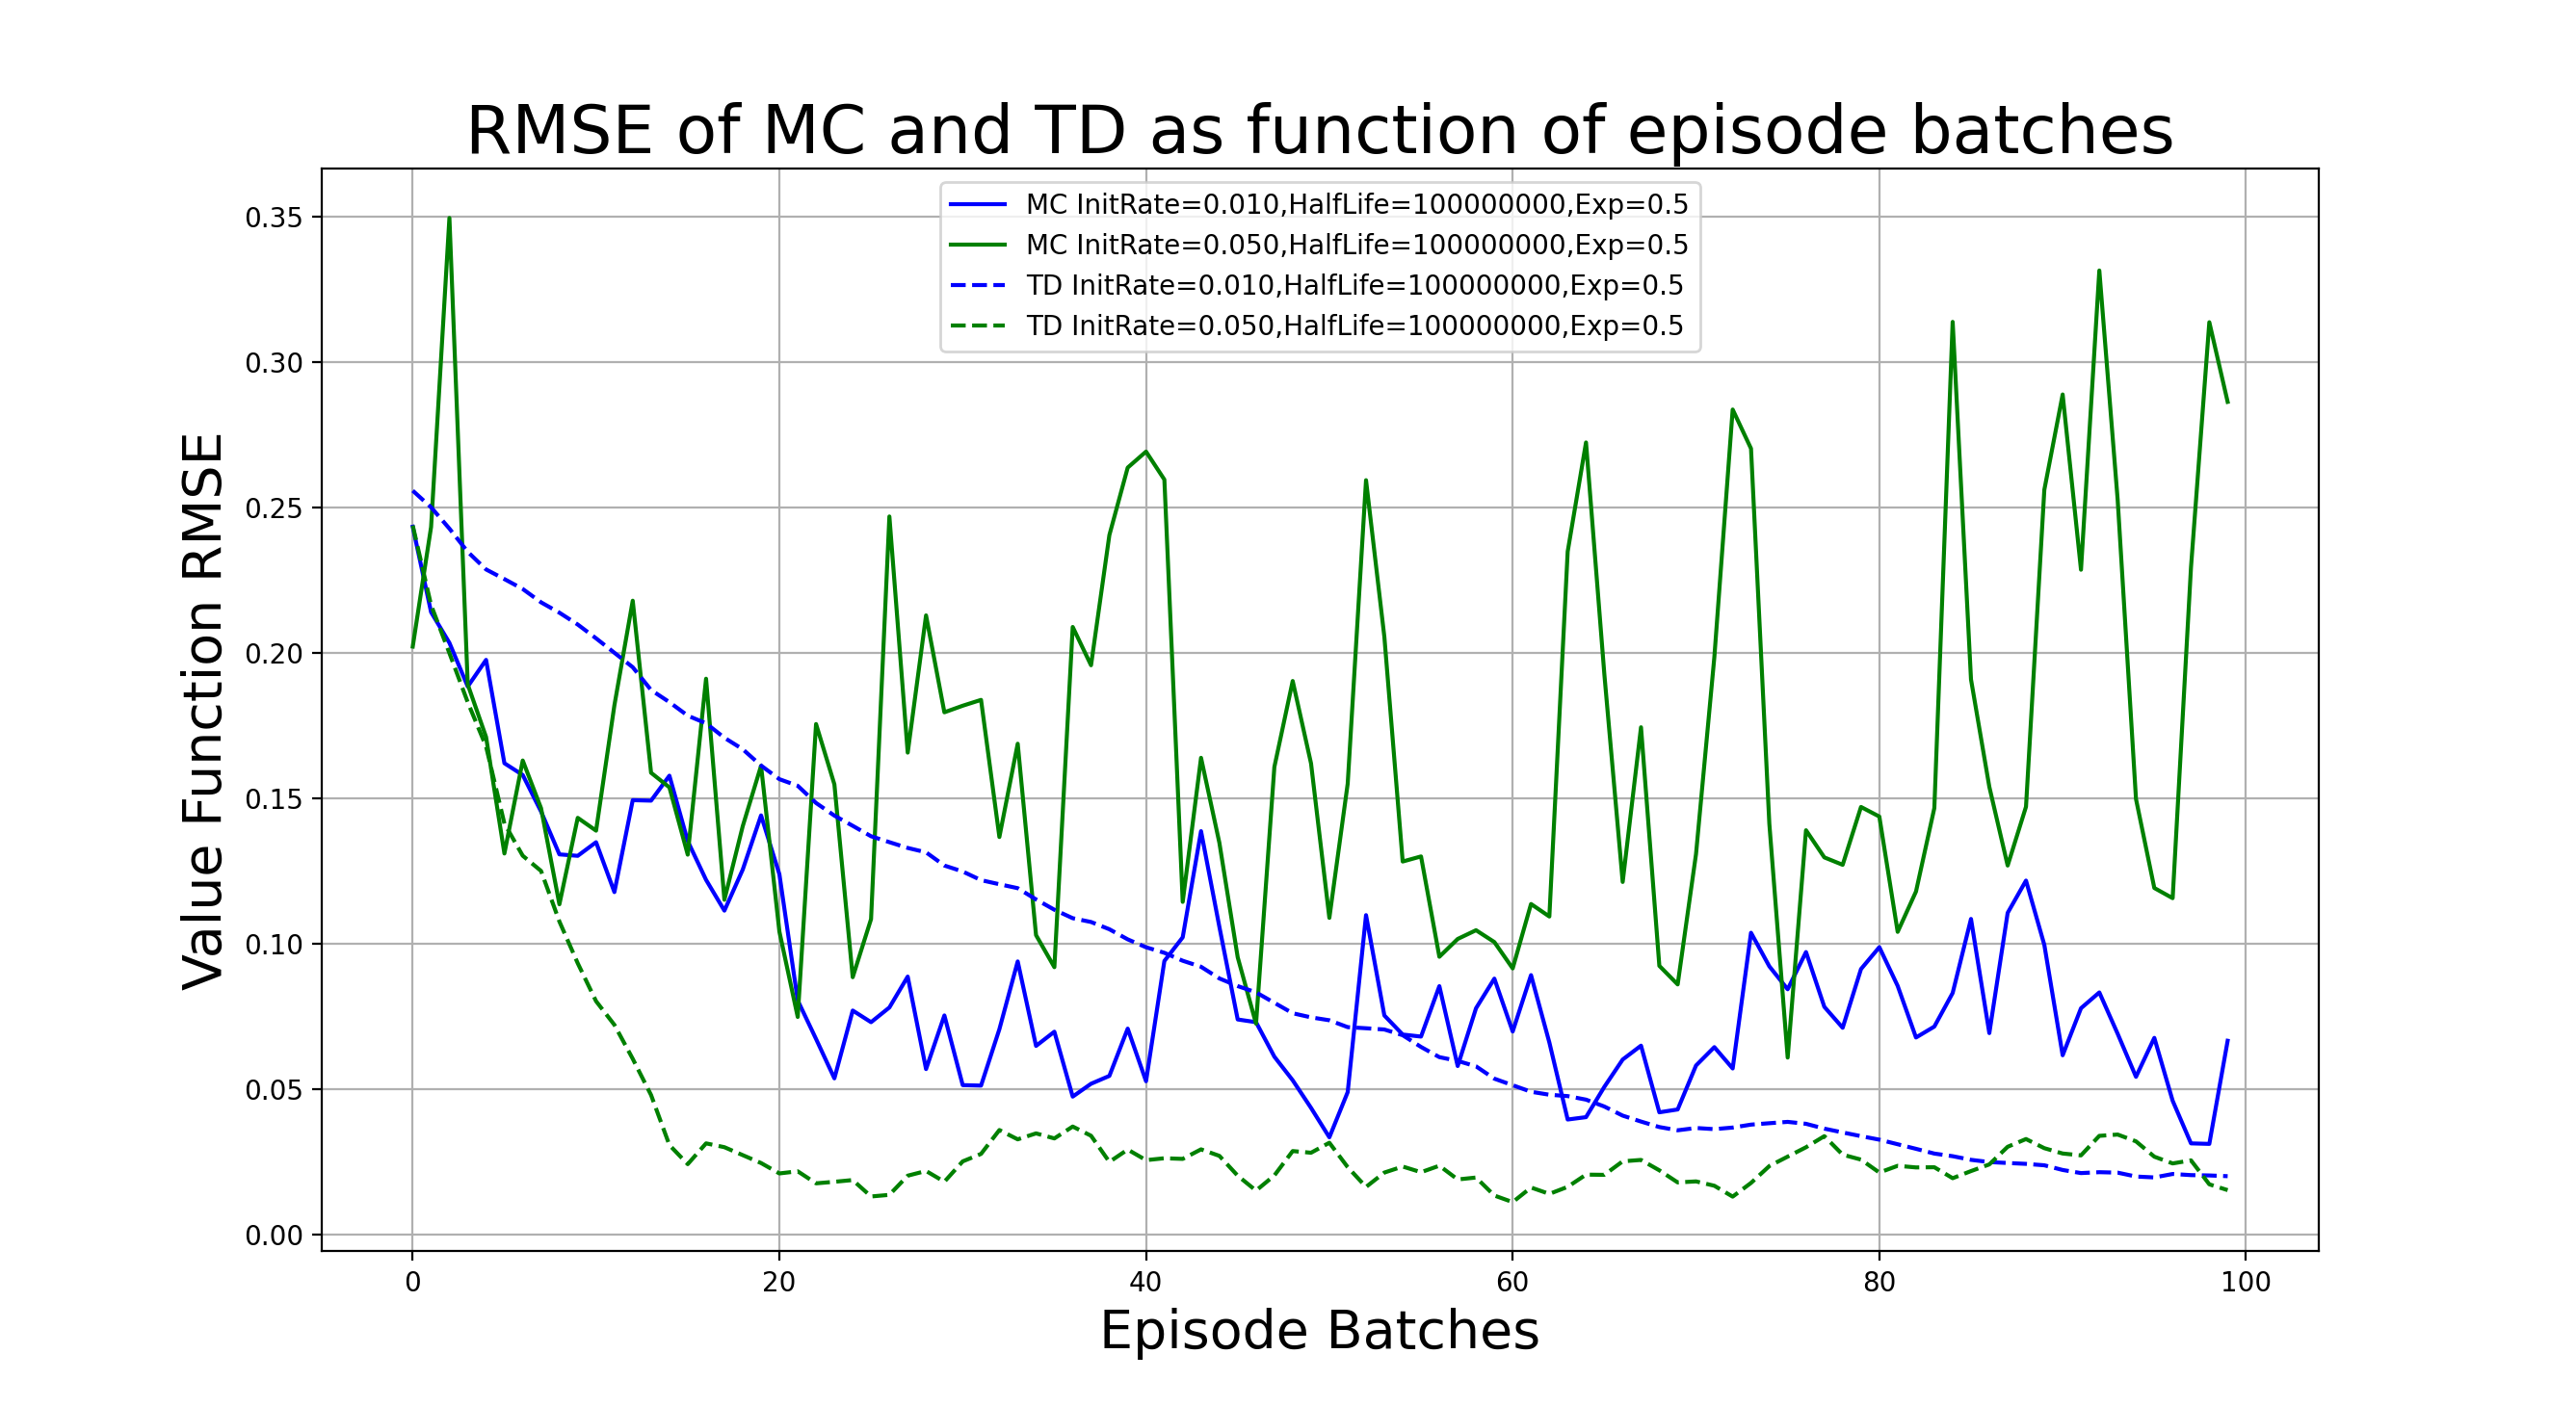
\includegraphics[width=12cm, height=7cm]{random_walk_mrp_convergence.png}
\end{frame}

\begin{frame}
\frametitle{RMSE of MC versus TD as function of episodes}
\pause
\begin{itemize}[<+->]
\item Symmetric random walk with barrier $B=10$ and no discounting
\item Graph depicts RMSE after every 7th episode (700 episodes in all)
\item Blue curves for constant $\alpha = 0.01$, green for constant $\alpha = 0.05$
\item Notice how MC has significantly more variance
\item RMSE progression is quite slow on blue curves (small learning rate)
\item MC progresses quite fast initially but then barely progresses
\item TD gets to fairly small RMSE quicker than corresponding MC
\item This performance of TD versus MC is typical for constant $\alpha$
\end{itemize}
\end{frame}

\begin{frame}[fragile]
\frametitle{Fixed-Data Experience Replay on TD versus MC}
\pause
\begin{itemize}[<+->]
\item So far, we've understood {\em how} TD learns versus {\em how} MC learns
\item Now we want to understand {\em what} TD learns versus {\em what} MC learns
\item To illustrate, we consider a finite set of trace experiences
\item The agent can tap into this finite set of traces experiences endlessly
\item But everything is ultimately sourced from this finite data set
\item So we'd end up tapping into these experiences repeatedly
\item We call this technique {\em Experience Replay}
\end{itemize}
\pause
\begin{lstlisting}
data: Sequence[Sequence[Tuple[str, float]]] = [
    [('A', 2.), ('A', 6.), ('B', 1.), ('B', 2.)],
    [('A', 3.), ('B', 2.), ('A', 4.), ('B', 2.), ('B', 0.)],
    [('B', 3.), ('B', 6.), ('A', 1.), ('B', 1.)],
    [('A', 0.), ('B', 2.), ('A', 4.), ('B', 4.), ('B', 2.), ('B', 3.)],
    [('B', 8.), ('B', 2.)]
]
\end{lstlisting}
\end{frame}

\begin{frame}
\frametitle{MC and TD learn different Value Functions}
\pause
\begin{itemize}[<+->]
\item It is quite obvious what MC Prediction algorithm would learn
\item MC Prediction is simply supervised learning with (state, return) pairs
\item But here those pairs ultimately come from the given finite pairs
\item So, MC estimates Value Function as average returns in the finite data
\item Running MC Prediction algo matches explicit average returns calc
\item But running TD Prediction algo gives significantly different answer
\item So what is TD Prediction algorithm learning?
\item TD drives towards VF of MRP {\em implied} by the finite experiences
\item Specifically, learns MLE for $\mathcal{P}_R$ from the given finite data
$$\mathcal{P}_R(s,r,s') = \frac {\sum_{i=1}^N \mathbb{I}_{S_i=s,R_{i+1}=r,S_{i+1}=s'}} {\sum_{i=1}^N \mathbb{I}_{S_i=s}}$$
\item TD is advantageous in Markov environments, MC in non-Markov
\end{itemize}
\end{frame}

\begin{frame}
\frametitle{Bootstrapping and Experiencing}
\pause
\begin{itemize}[<+->]
\item We summarize MC, TD and DP in terms of whether they:
\begin{itemize}[<+->]
\item Bootstrap:  Update to VF utilizes a current or prior estimate of the VF
\item Experience: Interaction with actual or simulated environment
\end{itemize}
\item TD and DP {\em do bootstrap} (updates use current/prior estimate of VF)
\item MC {\em does not bootstrap} (updates use trace experience returns)
\item MC and TD {\em do experience} (actual/simulated environment interaction)
\item DP {\em does not experience} (updates use transition probabilities)
\item Bootstrapping means backups are {\em shallow} (MC backups are {\em deep})
\item Experiencing means backups are {\em narrow} (DP backups are {\em wide})
\end{itemize}
\end{frame}


\begin{frame}
\frametitle{MC backup Diagram}
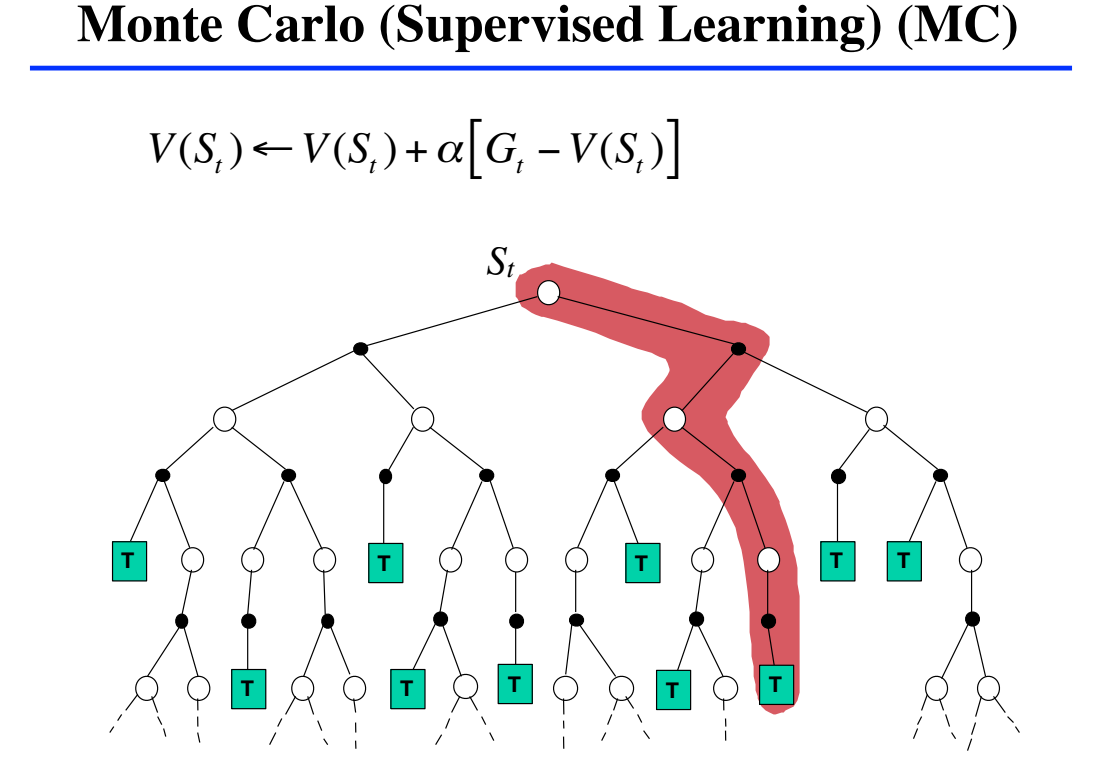
\includegraphics[width=12cm, height=7cm]{mc_backup.png}
\end{frame}

\begin{frame}
\frametitle{TD backup Diagram}
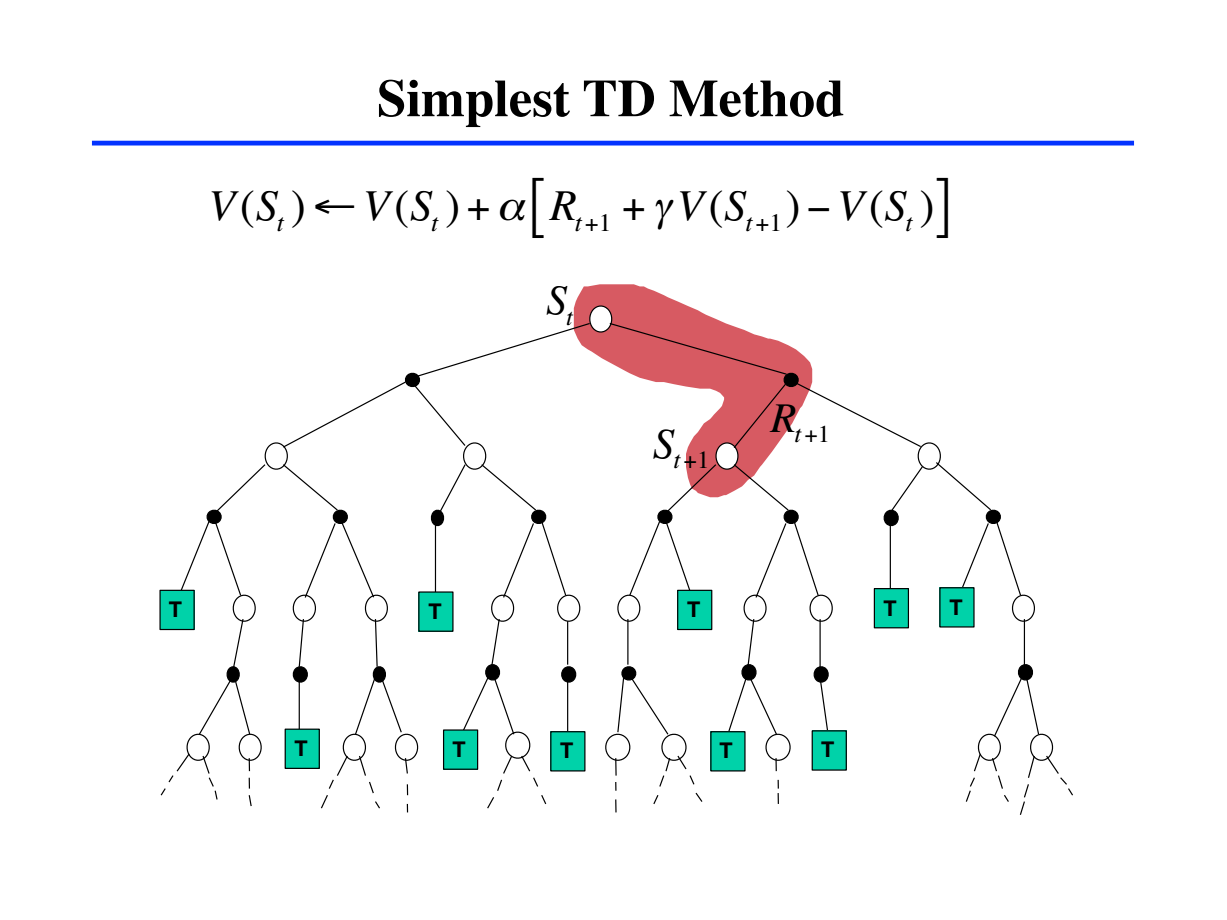
\includegraphics[width=12cm, height=7cm]{td_backup.png}
\end{frame}


\begin{frame}
\frametitle{DP backup Diagram}
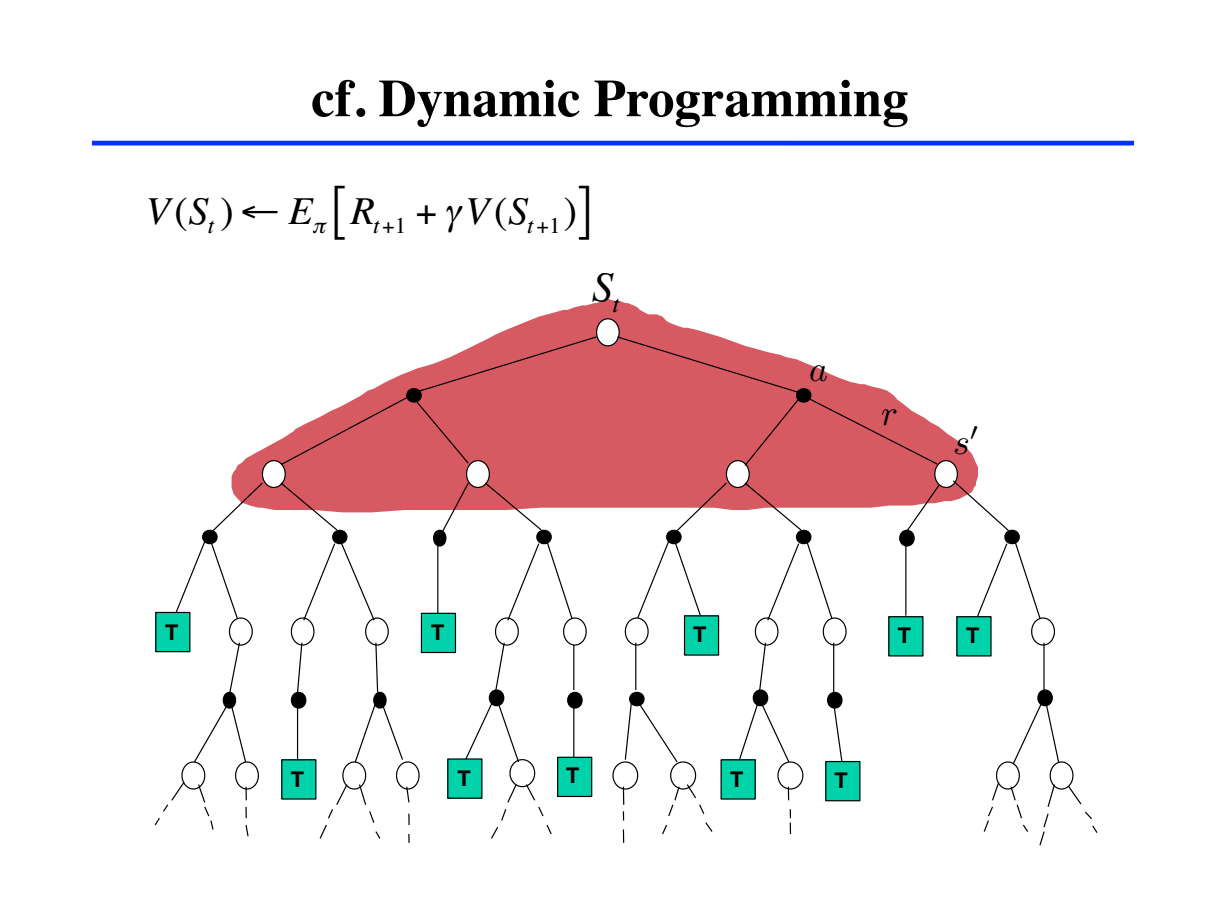
\includegraphics[width=12cm, height=7cm]{dp_backup.png}
\end{frame}

\begin{frame}
\frametitle{Unified View of RL}
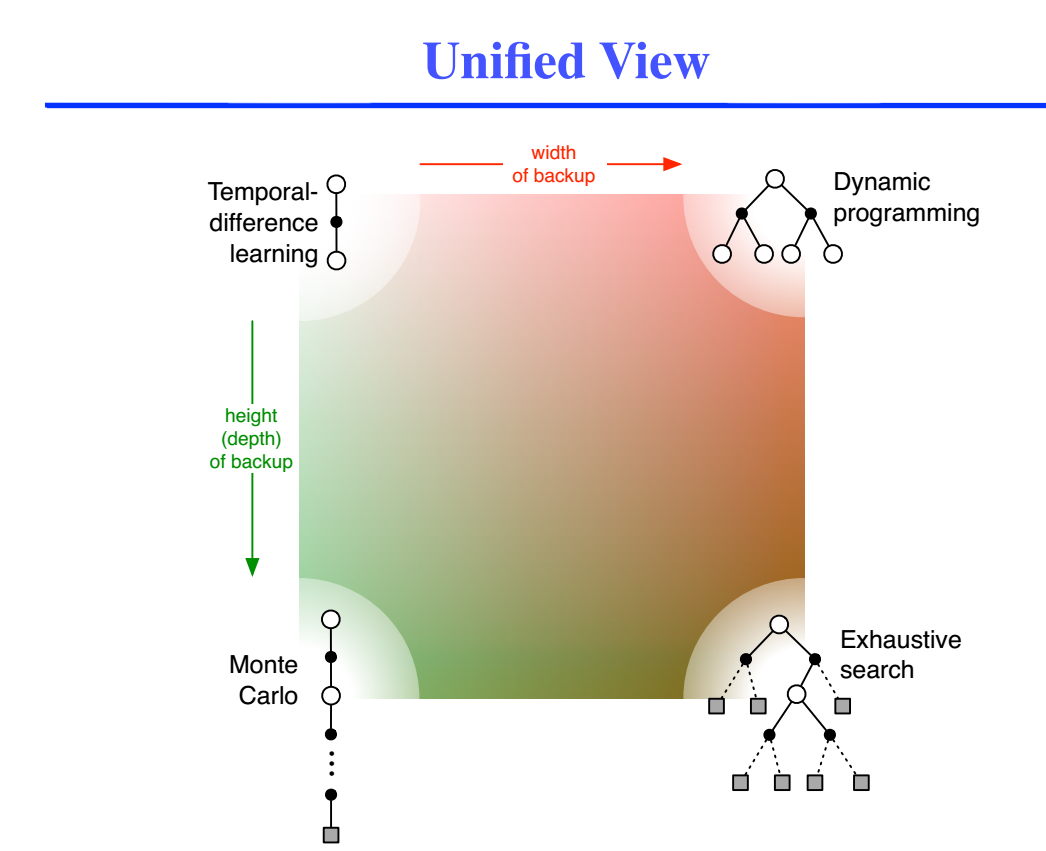
\includegraphics[width=12cm, height=7cm]{unified_view.png}
\end{frame}





\begin{frame}
\frametitle{Tabular $n$-step Bootstrapping}
\pause
\begin{itemize}[<+->]
\item Tabular TD Prediction bootstraps the Value Function with update:
$$V(S_t) \leftarrow V(S_t) + \alpha \cdot (R_{t+1} + \gamma \cdot V(S_{t+1}) - V(S_t))$$
\item So it's natural to extend this to bootstrapping with 2 steps ahead:
$$V(S_t) \leftarrow V(S_t) + \alpha \cdot (R_{t+1} + \gamma \cdot R_{t+2} + \gamma^2 \cdot V(S_{t+2})- V(S_t))$$
\item Generalize to bootstrapping with $n \geq 1$ time steps ahead:
$$V(S_t) \leftarrow V(S_t) + \alpha \cdot (G_{t,n} - V(S_t))$$
\item $G_{t,n}$ (known as $n$-step bootstrapped return) is defined as:
\begin{align*}
G_{t,n} & = \sum_{i=t+1}^{t+n} \gamma^{i-t-1} \cdot R_i  + \gamma^n \cdot V(S_{t+n}) \\
& = R_{t+1} + \gamma \cdot R_{t+2} + \gamma^2 \cdot R_{t+3} + \ldots + \gamma^{n-1} \cdot R_{t+n} + \gamma^n \cdot V(S_{t+n})
\end{align*}
\end{itemize}
\end{frame}

\begin{frame}
\frametitle{$n$-step Bootstrapping with Function Approximation}
\pause
\begin{itemize}[<+->]
\item Generalizing this to the case of Function Approximation, we get:
$$\Delta \bm{w} = \alpha \cdot (G_{t,n} - V(S_t; \bm{w})) \cdot \nabla_{\bm{w}} V(S_t;\bm{w})$$
\item This looks similar to formula for parameters update for MC and TD
\item In terms of conceptualizing the change in parameters as product of:
\begin{itemize}[<+->]
\item {\em Learning Rate} $\alpha$
\item {\em $n$-step Bootstrapped Error} $G_{t,n} - V(S_t; \bm{w})$
\item {\em Estimate Gradient} of the conditional expected return $V(S_t;\bm{w})$ with respect to the parameters $\bm{w}$
\end{itemize}
\item $n$ serves as a parameter taking us across the spectrum from TD to MC
\item $n=1$ is the case of TD while sufficiently large $n$ is the case of MC
\end{itemize}
\end{frame}

\begin{frame}
\frametitle{$\lambda$-Return Prediction Algorithm}
\pause
\begin{itemize}[<+->]
\item Instead of $G_{t,n}$, a valid target is a weighted-average target:
$$\sum_{n=1}^N u_n \cdot G_{t,n} + u \cdot G_t \text{ where } u + \sum_{n=1}^N u_n = 1$$
\item Any of the $u_n$ or $u$ can be 0, as long as they all sum up to 1
\item The $\lambda$-Return target is a special case of weights $u_n$ and $u$
$$u_n = (1 - \lambda) \cdot \lambda^{n-1} \text{ for all } n = 1, \ldots, T-t-1$$
$$u_n = 0 \text{ for all } n \geq T-t \text{ and } u = \lambda^{T-t-1}$$
\item We denote the $\lambda$-Return target as $G_t^{(\lambda)}$, defined as:
$$G_t^{(\lambda)} = (1-\lambda) \cdot \sum_{n=1}^{T-t-1} \lambda^{n-1} \cdot G_{t,n} + \lambda^{T-t-1} \cdot G_t$$
$$\Delta \bm{w} = \alpha \cdot (G_t^{(\lambda)} - V(S_t; \bm{w})) \cdot \nabla_{\bm{w}} V(S_t;\bm{w})$$
\end{itemize}
\end{frame}

\begin{frame}
\frametitle{Online versus Offline}
\pause
\begin{itemize}[<+->]
\item Note that for $\lambda=0$, the $\lambda$-Return target reduces to the TD target
\item Note that for $\lambda=1$, the $\lambda$-Return target reduces to the MC target $G_t$
\item $\lambda$ parameter enables us to finely tune from TD ($\lambda=0$) to MC ($\lambda=1$)
\item Note that for $\lambda > 0$, updates are made only at the end of an episode
\item Algorithms updating at end of episodes known as {\em Offline Algorithms}
\item Online algorithms (updates after each time step) are appealing:
\begin{itemize}[<+->]
\item Updated VF can be utilized immediately for next time step's update
\item This facilitates continuous/fast learning
\end{itemize}
\item Can we have a similar $\lambda$-tunable online algorithm for Prediction?
\item Yes - this is known as the TD($\lambda$) Prediction algorithm
\end{itemize}
\end{frame}

\begin{frame}
\frametitle{Memory Function}
\pause
\begin{itemize}[<+->]
\item TD($\lambda$) algorithm is based on the concept of {\em Eligibility Traces}
\item We introduce the concept by defining a {\em Memory Function} $M(t)$
\item Assume an event occurs at times $t_1 < t_2 < \ldots < t_n \in \mathbb{R}_{\geq 0}$
\item We want $M(t)$ to remember the \# of times the event has occurred
\item But we also want it to have an element of ``forgetfulness''
\item Recent event-occurrences remembered better than older occurrences
\item  We want $M(\cdot)$ to give us a time-decayed count of event-occurrences
\begin{equation*}
M(t) = 
\begin{cases}
\mathbb{I}_{t=t_1} & \text{ if } t \leq t_1, \\
M(t_i) \cdot \theta^{t - t_i} + \mathbb{I}_{t=t_{i+1}}& \text{ if }  t_i < t \leq t_{i+1} \text{ for any } 1 \leq i < n, \\
M(t_n) \cdot \theta^{t - t_n} & \text{ otherwise (i.e., } t > t_n)
\end{cases}
\end{equation*}
\item There's an uptick of 1 each time the event occurs, but it decays by a factor of $\theta^{\Delta t}$ over any interval $\Delta t$ where the event doesn't occur
\item Thus, $M(\cdot)$ captures the notion of frequency as well as recency
\end{itemize}
\end{frame}

\begin{frame}
\frametitle{Memory Function with $\theta = 0.8$}
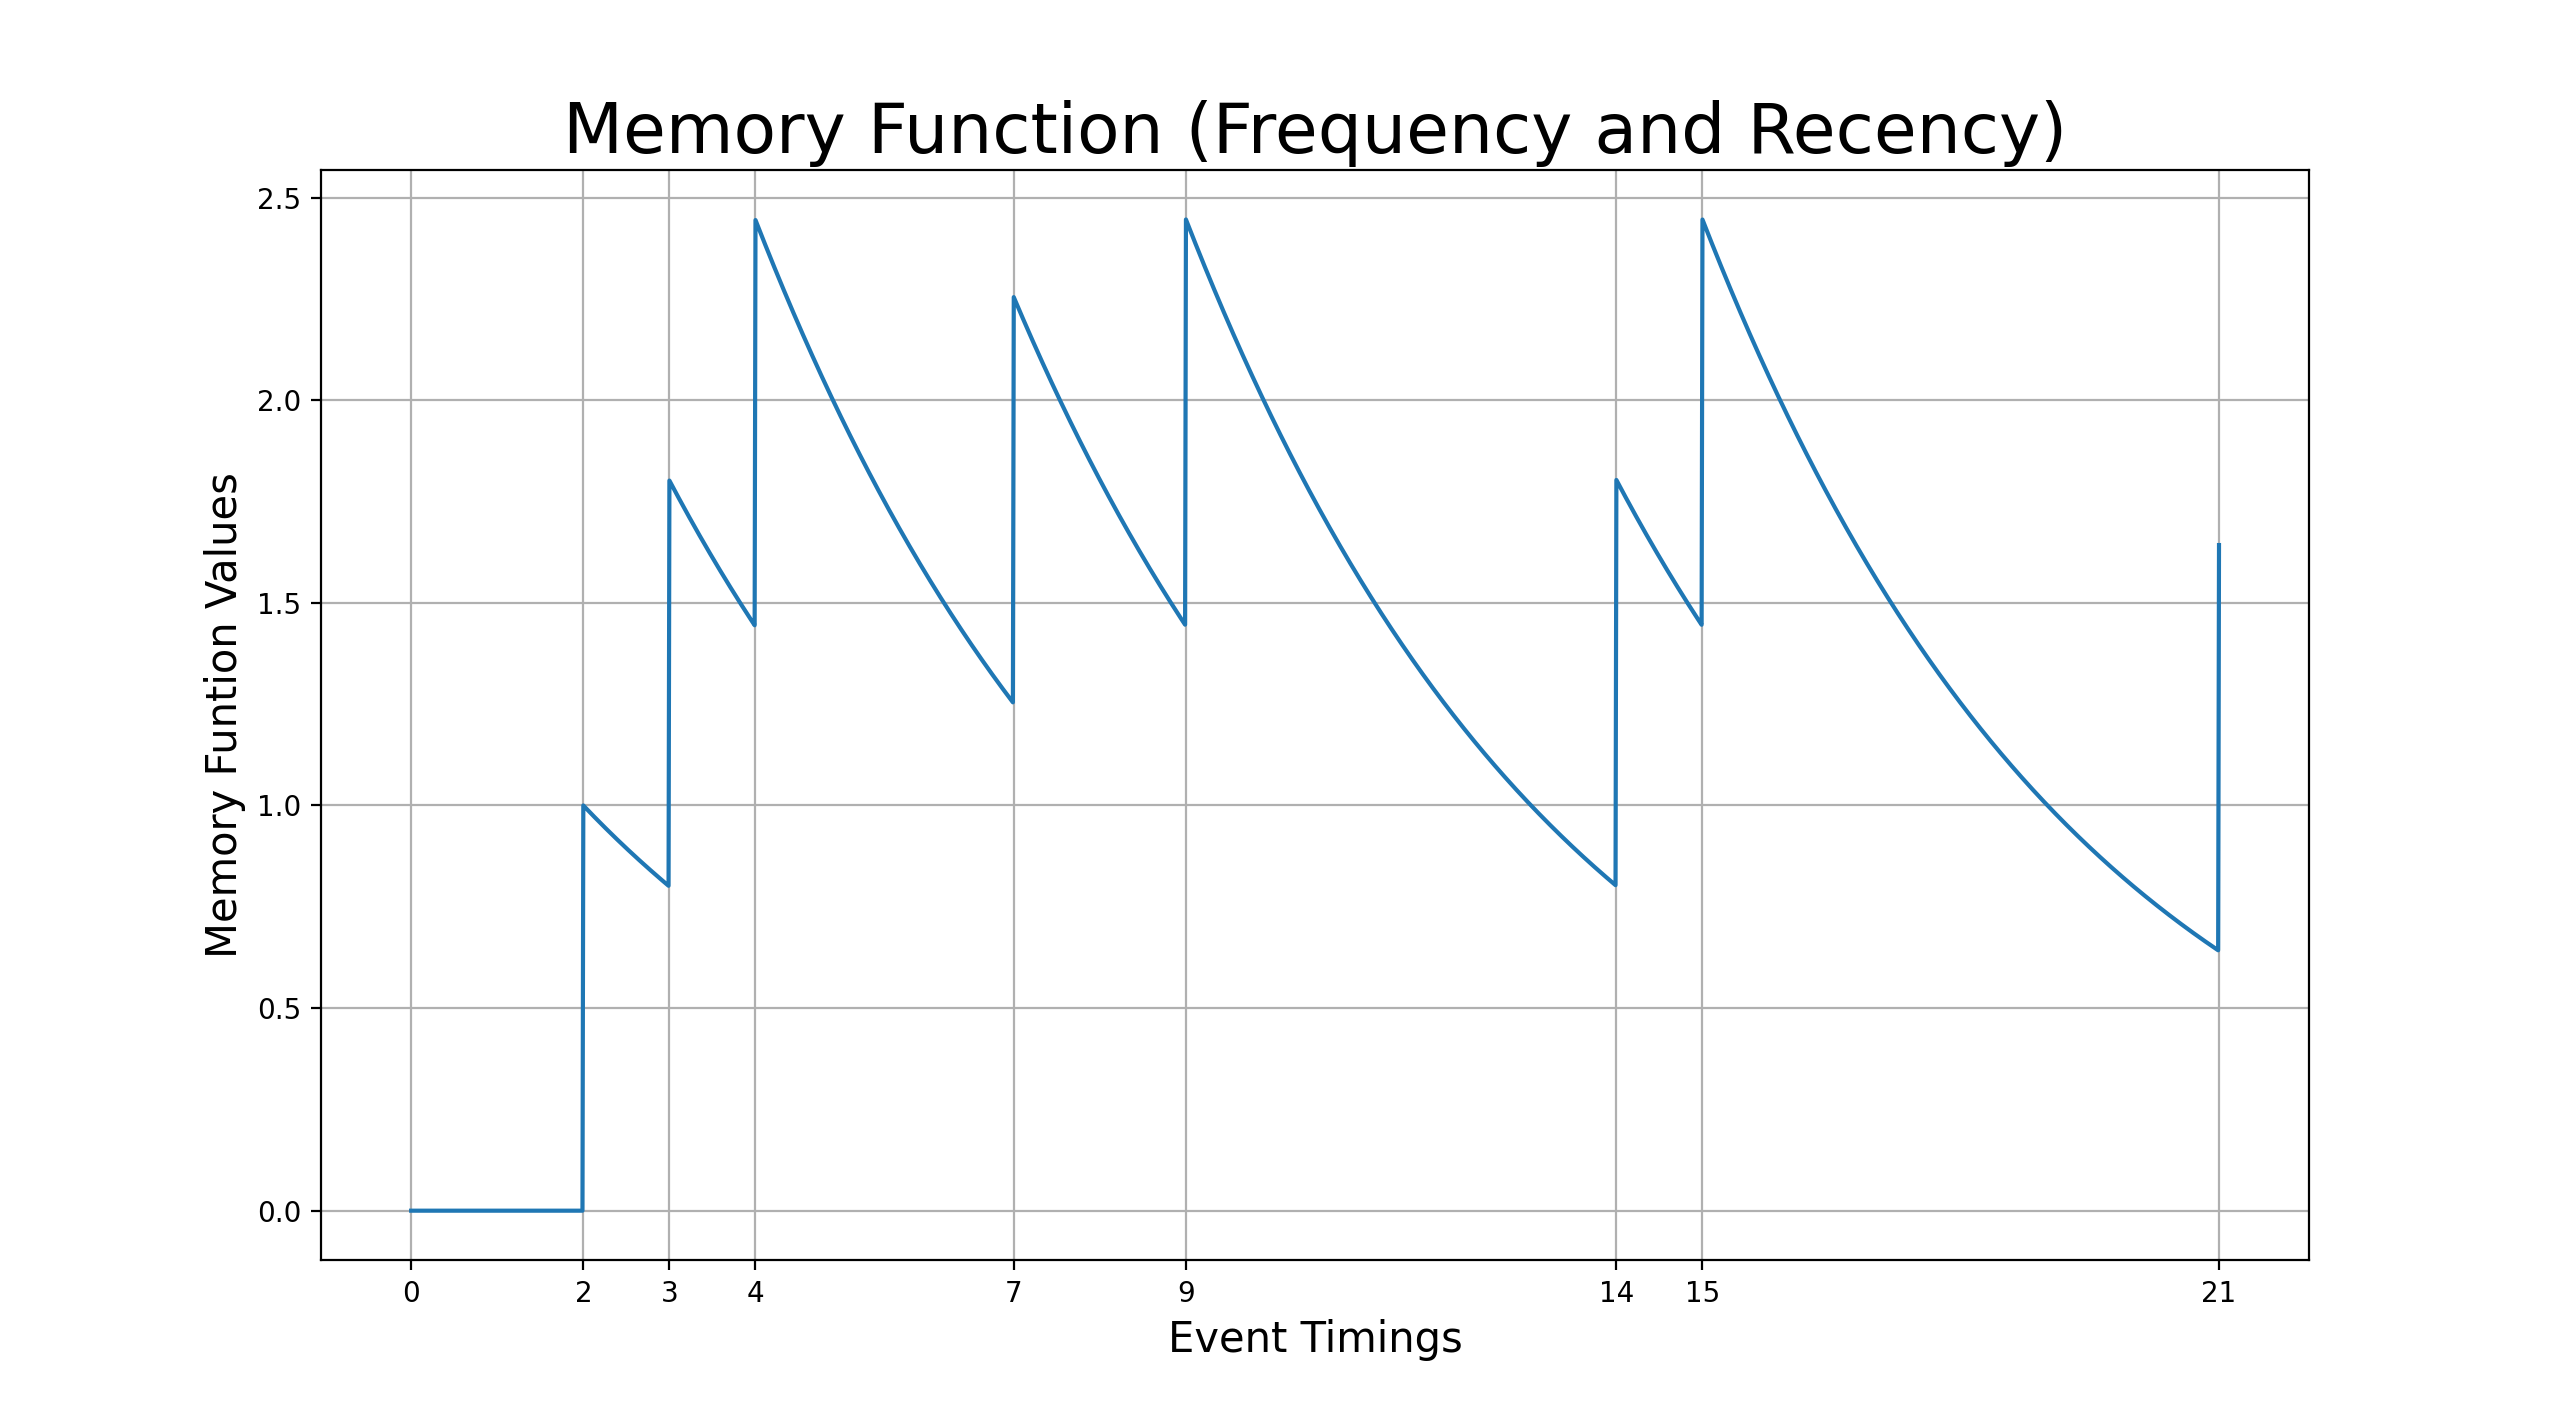
\includegraphics[width=12cm, height=7cm]{memory_function.png}
\end{frame}


\begin{frame}
\frametitle{Eligibility Traces and Tabular TD($\lambda)$ Prediction}
\pause
\begin{itemize}[<+->]
\item Assume a finite state space with non-terminals $\mathcal{N} = \{s_1, s_2, \ldots, s_m\}$
\item Eligibility Trace for each state $s\in S$ is defined as the Memory function $M(\cdot)$ with $\theta = \gamma \cdot \lambda$, and the event timings are the time steps at which the state $s$ occurs in a trace experience
 \item Eligibility trace for a given trace experience at time $t$ is a function
$$E_t: \mathcal{N} \rightarrow \mathbb{R}_{\geq 0}$$
$$E_0(s) = 0, \text{ for all } s \in \mathcal{N}$$
$$E_t(s) = \gamma \cdot \lambda \cdot E_{t-1}(s) + \mathbb{I}_{S_t=s}, \text{ for all } s \in \mathcal{N}, \text{ for all } t = 1, 2, \ldots$$
\item Tabular TD($\lambda$) Prediction algorithm performs following update at each time step $t$ in each trace experience:
$$V(s) \leftarrow V(s) + \alpha \cdot (R_{t+1} + \gamma \cdot V(S_{t+1}) - V(S_t)) \cdot E_t(s), \text{ {\em for all} } s \in \mathcal{N}$$
\end{itemize}
\end{frame}

\begin{frame}
\frametitle{``Equivalence'' of TD($\lambda)$ and $\lambda$-Return}
\pause
\begin{itemize}[<+->]
\item TD($\lambda$) is an online algorithm, similar to TD
\item But unlike TD, we update the VF {\em for all} states at each time step
\item VF update for each state is proportional to TD-Error $\delta_t$ (like TD)
 \item But here, $\delta_t$ is scaled by $E_t(s)$ for each state $s$ at each $t$
$$V(s) \leftarrow V(s) + \alpha \cdot \delta_t \cdot E_t(s), \text{ {\em for all} } s \in \mathcal{N}$$
\item But how is TD($\lambda)$ Prediction linked to the $\lambda$-Return Prediction?
\item It turns out that if we made all updates in an offline manner, then sum of updates for a fixed state $s \in \mathcal{N}$ over entire trace experience equals (offline) update for $s$ in the $\lambda$-Return prediction algorithm
\end{itemize}
\pause
\begin{theorem}
$$\sum_{t=0}^{T-1} \alpha \cdot \delta_t \cdot E_t(s) = \sum_{t=0}^{T-1} \alpha \cdot (G_t^{(\lambda)} - V(S_t)) \cdot \mathbb{I}_{S_t=s}, \text{ for all } s \in \mathcal{N}$$
\end{theorem}
\end{frame}


\begin{frame}
\frametitle{Proof}
\pause

\begin{equation*}
\begin{aligned}[b]
G_t^{(\lambda)} =  & (1 - \lambda) \cdot \lambda^0 \cdot (R_{t+1} + \gamma \cdot V(S_{t+1})) \\
+ & (1 - \lambda) \cdot \lambda^1 \cdot (R_{t+1} + \gamma \cdot R_{t+2} + \gamma^2 \cdot V(S_{t+2})) \\
+ & (1 - \lambda) \cdot \lambda^2 \cdot (R_{t+1} + \gamma \cdot R_{t+2} + \gamma^2 \cdot R_{t+3} + \gamma^3 \cdot V(S_{t+2})) \\
+ & \ldots \\
\pause
= & (\gamma \lambda)^0 \cdot (R_{t+1} + \gamma \cdot V(S_{t+1}) - \gamma \lambda \cdot V(S_{t+1})) \\
+ & (\gamma \lambda)^1 \cdot (R_{t+2} + \gamma \cdot V(S_{t+2}) - \gamma \lambda \cdot V(S_{t+2})) \\
+ & (\gamma \lambda)^2 \cdot (R_{t+3} + \gamma \cdot V(S_{t+3}) - \gamma \lambda \cdot V(S_{t+3})) \\
+ & \ldots
\end{aligned}
\end{equation*}
\end{frame}


\begin{frame}
\frametitle{Proof}
\pause

\begin{equation*}
\begin{aligned}[b]
G_t^{(\lambda)} =  & (\gamma \lambda)^0 \cdot (R_{t+1} + \gamma \cdot V(S_{t+1}) - \gamma \lambda \cdot V(S_{t+1})) \\
+ & (\gamma \lambda)^1 \cdot (R_{t+2} + \gamma \cdot V(S_{t+2}) - \gamma \lambda \cdot V(S_{t+2})) \\
+ & (\gamma \lambda)^2 \cdot (R_{t+3} + \gamma \cdot V(S_{t+3}) - \gamma \lambda \cdot V(S_{t+3})) \\
+ & \ldots
\end{aligned}
\end{equation*}

\begin{equation*}
\begin{aligned}[b]
G_t^{(\lambda)} - V(S_t) = & (\gamma \lambda)^0 \cdot (R_{t+1} + \gamma \cdot V(S_{t+1}) - V(S_t)) \\
+ & (\gamma \lambda)^1 \cdot (R_{t+2} + \gamma \cdot V(S_{t+2}) - V(S_{t+1})) \\
+ & (\gamma \lambda)^2 \cdot (R_{t+3} + \gamma \cdot V(S_{t+3}) - V(S_{t+2})) \\
+ & \ldots \\
= & \delta_t + \gamma \lambda \cdot \delta_{t+1} + (\gamma \lambda)^2 \cdot \delta_{t+2} + \ldots
\end{aligned}
\end{equation*}
\end{frame}

\begin{frame}
\frametitle{Proof}
\pause
Now assume that a specific non-terminal state $s$ appears at time steps $t_1, t_2, \ldots, t_n$. Then,
\begin{align*}
\sum_{t=0}^{T-1} \alpha \cdot (G_t^{(\lambda)} - V(S_t)) \cdot \mathbb{I}_{S_t=s} & = \sum_{i=1}^n \alpha \cdot (G_{t_i}^{(\lambda)} - V(S_{t_i})) \\
& = \sum_{i=1}^n \alpha \cdot (\delta_{t_i} + \gamma \lambda \cdot \delta_{t_i+1} + (\gamma \lambda)^2 \cdot \delta_{t_i+2} + \ldots ) \\
& = \sum_{t=0}^{T-1} \alpha \cdot \delta_t \cdot E_t(s)
\end{align*}
\qed
\end{frame}


\begin{frame}
\frametitle{TD(0) and TD(1) with Offline Updates}
\pause
\begin{itemize}[<+->]
\item To be clear, TD($\lambda$) Prediction is an online algorithm
\item So {\em not the same} as {\em offline} $\lambda$-Return Prediction
\item If we modified TD($\lambda$) to be offline, they'd be equivalent
\item Offline version of TD($\lambda$) would not update VF at each step
\item Accumulate changes in buffer, update VF offline with buffer contents
\item If we set $\lambda = 0$, $E_t(s) = \mathbb{I}_{S_t=s}$ and so, the update reduces to:
$$V(S_t) \leftarrow V(S_t) + \alpha \cdot \delta_t$$
\item This is exactly the TD update. So, TD is often refered to as TD(0)
\item If we set $\lambda=1$ with episodic traces, sum of all VF updates for a state over a trace experience is equal to it's VF update in Every-Visit MC
\item Hence, Offline TD(1) is equivalent to Every-Visit MC
\end{itemize}
\end{frame}

\begin{frame}
\frametitle{TD($\lambda$) Prediction with Function Approximation}
\pause
\begin{itemize}[<+->]
\item Generalize TD($\lambda$) to the case of function approximation
\item Data-Type of eligibility traces same as func-approx parameters $\bm{w}$
\item So here we denote eligibility traces at time $t$ as simply $\bm{E}_t$
\item Initialize $\bm{E}_0$ to 0 for each component in it's data type
\item For each time step $t > 0$, $\bm{E}_t$ is calculated recursively:
$$\bm{E}_t = \gamma \lambda \cdot \bm{E}_{t-1} + \nabla_{\bm{w}} V(S_t;\bm{w})$$
\item VF approximation update at each time step $t$ is as follows:
$$\Delta \bm{w} = \alpha \cdot (R_{t+1} + \gamma \cdot V(S_{t+1}; \bm{w}) - V(S_t; \bm{w})) \cdot \bm{E}_t$$
\item Expressed more succinctly in terms of function-approx TD-Error $\delta_t$:
$$\Delta \bm{w} = \alpha \cdot \delta_t \cdot \bm{E}_t$$
\end{itemize}
\end{frame}


\begin{frame}
\frametitle{Key Takeaways from this Chapter}
\pause
\begin{itemize}[<+->]
\item Bias-Variance tradeoff of TD versus MC
\item MC learns the mean of the observed returns while TD learns something "deeper" - it implicitly estimates an MRP from given data and produces the Value Function of the implicitly-estimated MRP
\item Understanding TD versus MC versus DP from the perspectives of:
\begin{itemize}[<+->]
\item ``Bootstrapping''
\item ``Experiencing''
\end{itemize}
\item ``Equivalence'' of $\lambda$-Return Prediction and TD($\lambda$) Prediction
\item TD is equivalent to TD(0) and MC is ``equivalent'' to TD(1)
\end{itemize}
\end{frame}


\end{document}